\section{Resultados}
%------------------------------------------------

\begin{frame}{Resultados}
    \Huge{\centerline{\textbf{Resultados}}}
\end{frame}


\begin{frame}{Resultados}

        \begin{center}
        \begin{figure}
        \caption{Dados experimentais obtidos, curva Diametros [cm] $\times$ $V$ (Tensão) em [Volts], do primeiro padrão de Difração.}
        \vspace*{-0.25cm}
        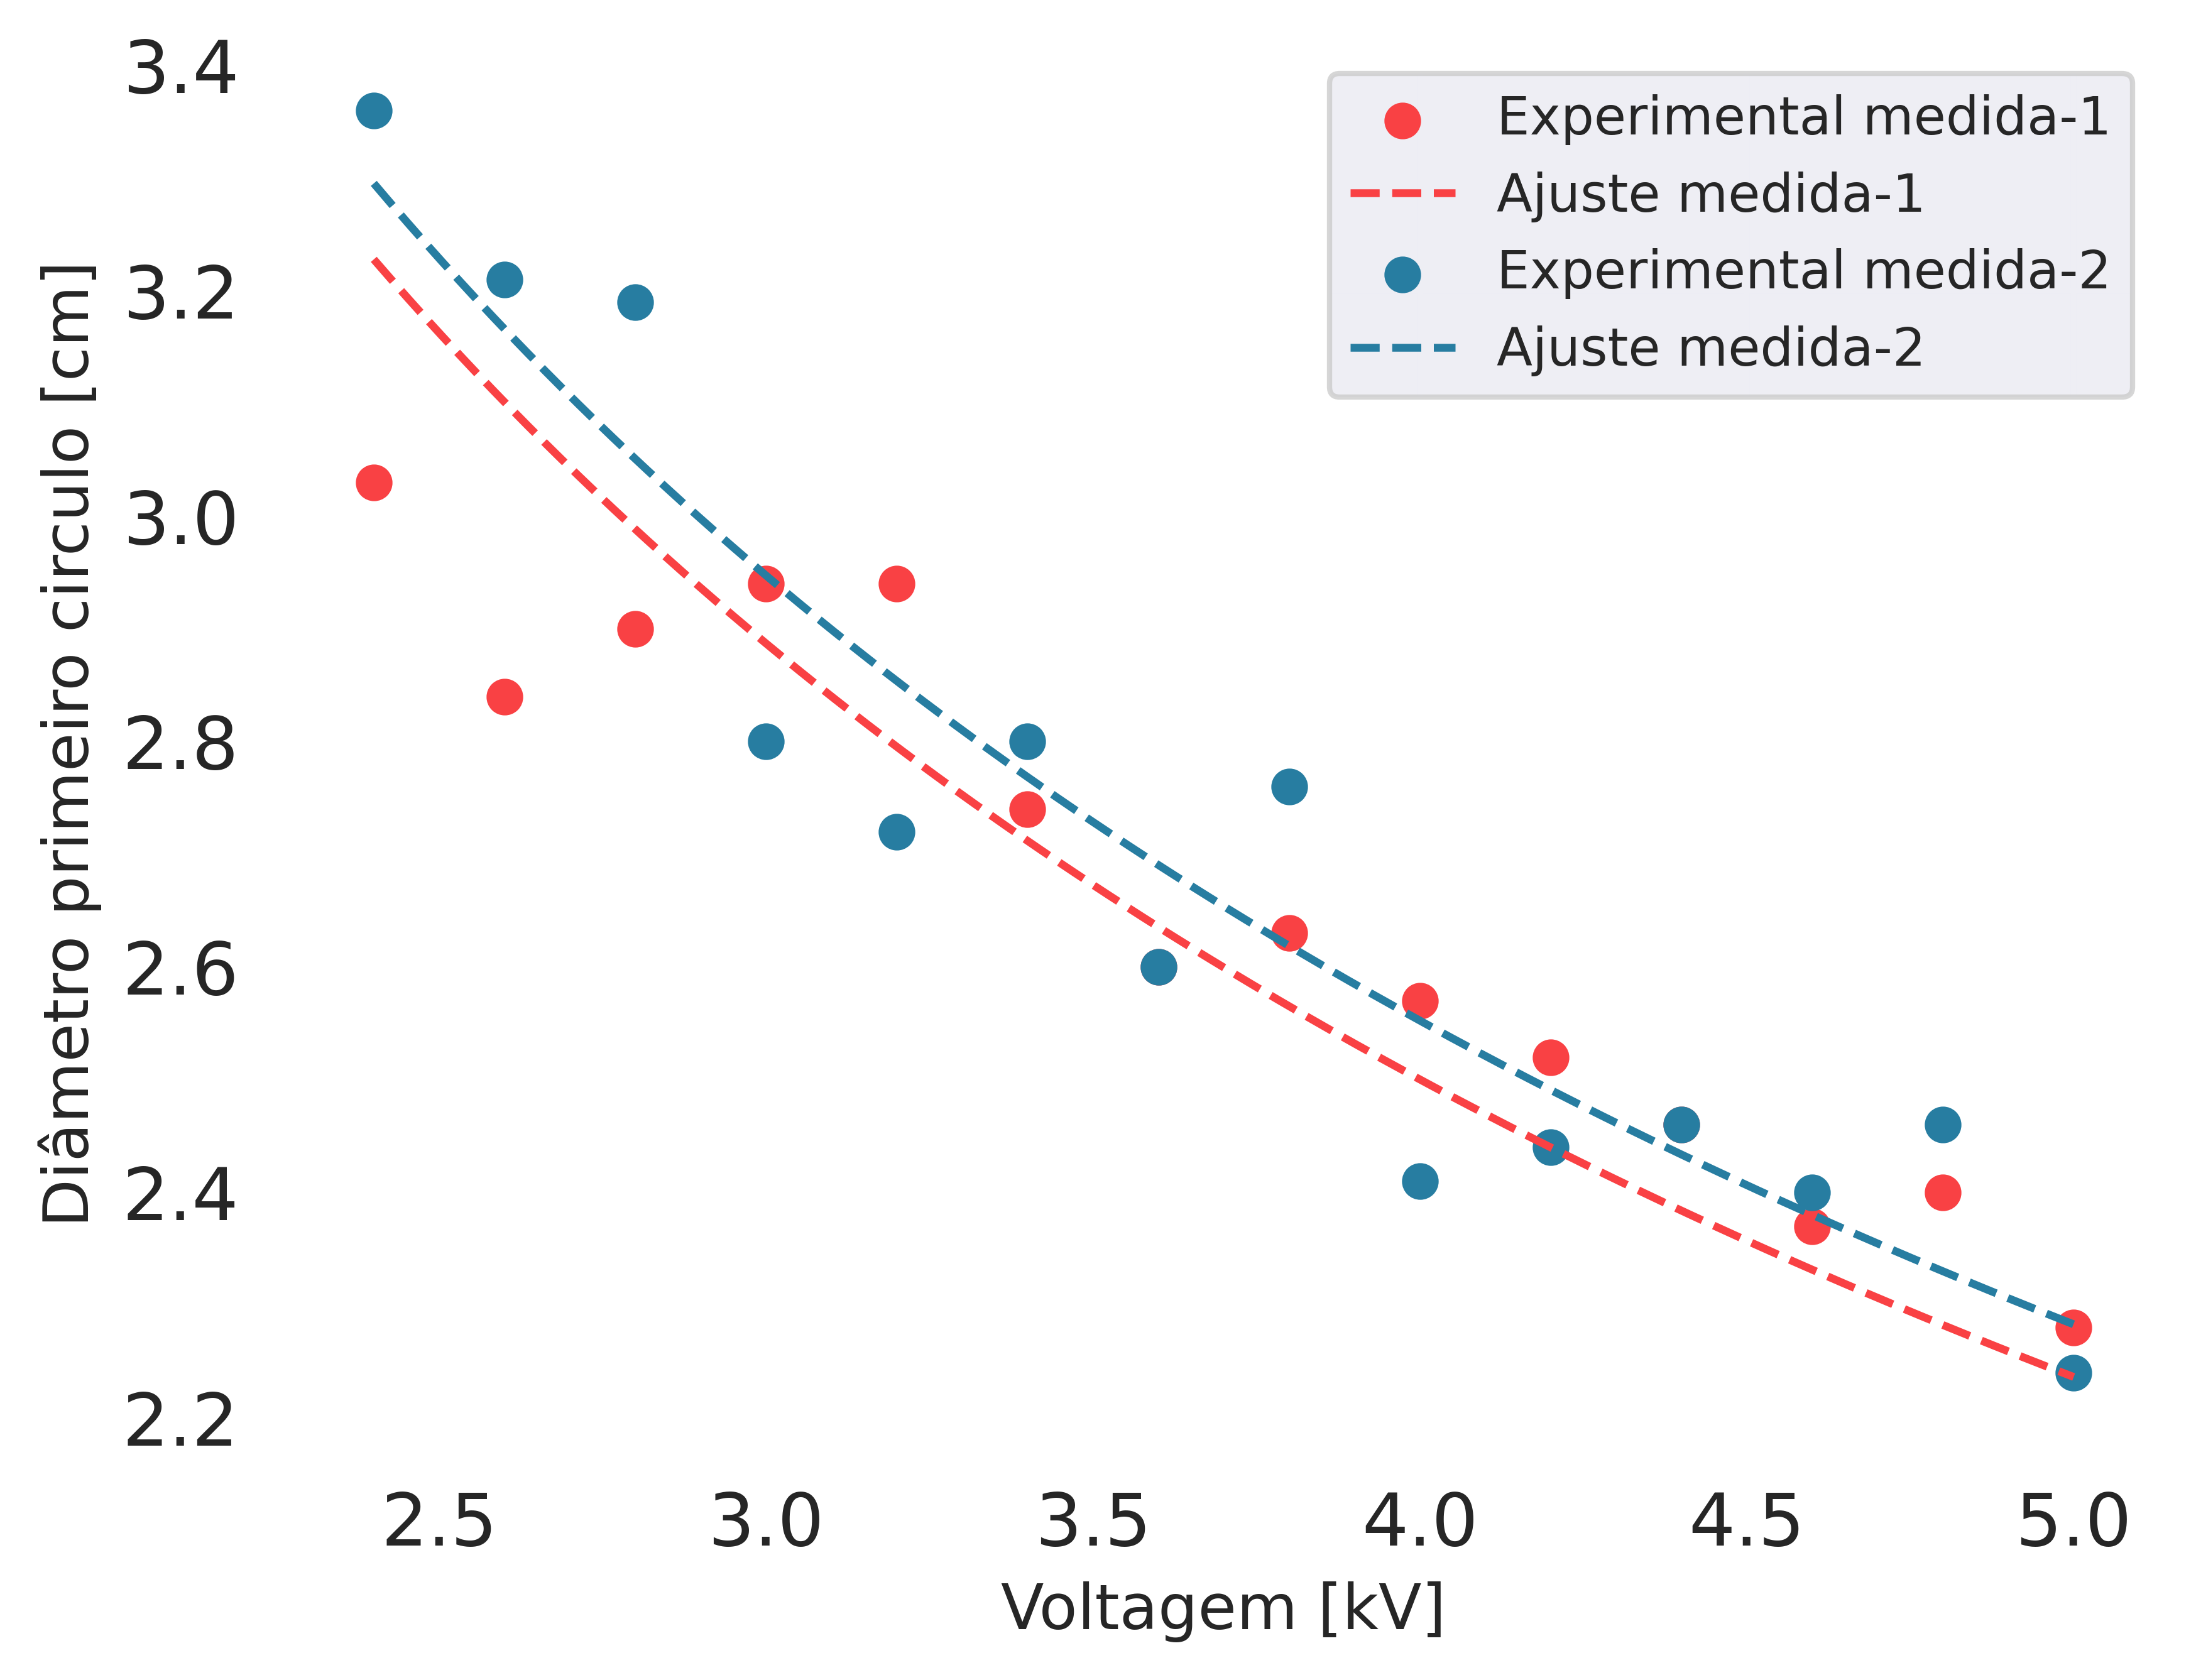
\includegraphics[width=0.75\textwidth,height=0.75\textheight,keepaspectratio]{figuras/fit1.png}\par
        {\scriptsize Fonte: Elabora pelo autor.}
        \end{figure}
        \end{center}
    
\end{frame}

\begin{frame}{Resultados}

        \begin{center}
        \begin{figure}
        \caption{Dados experimentais obtidos, curva Diametros [cm] $\times$ $V$ (Tensão) em [Volts], do segundo padrão de Difração.}
        \vspace*{-0.25cm}
        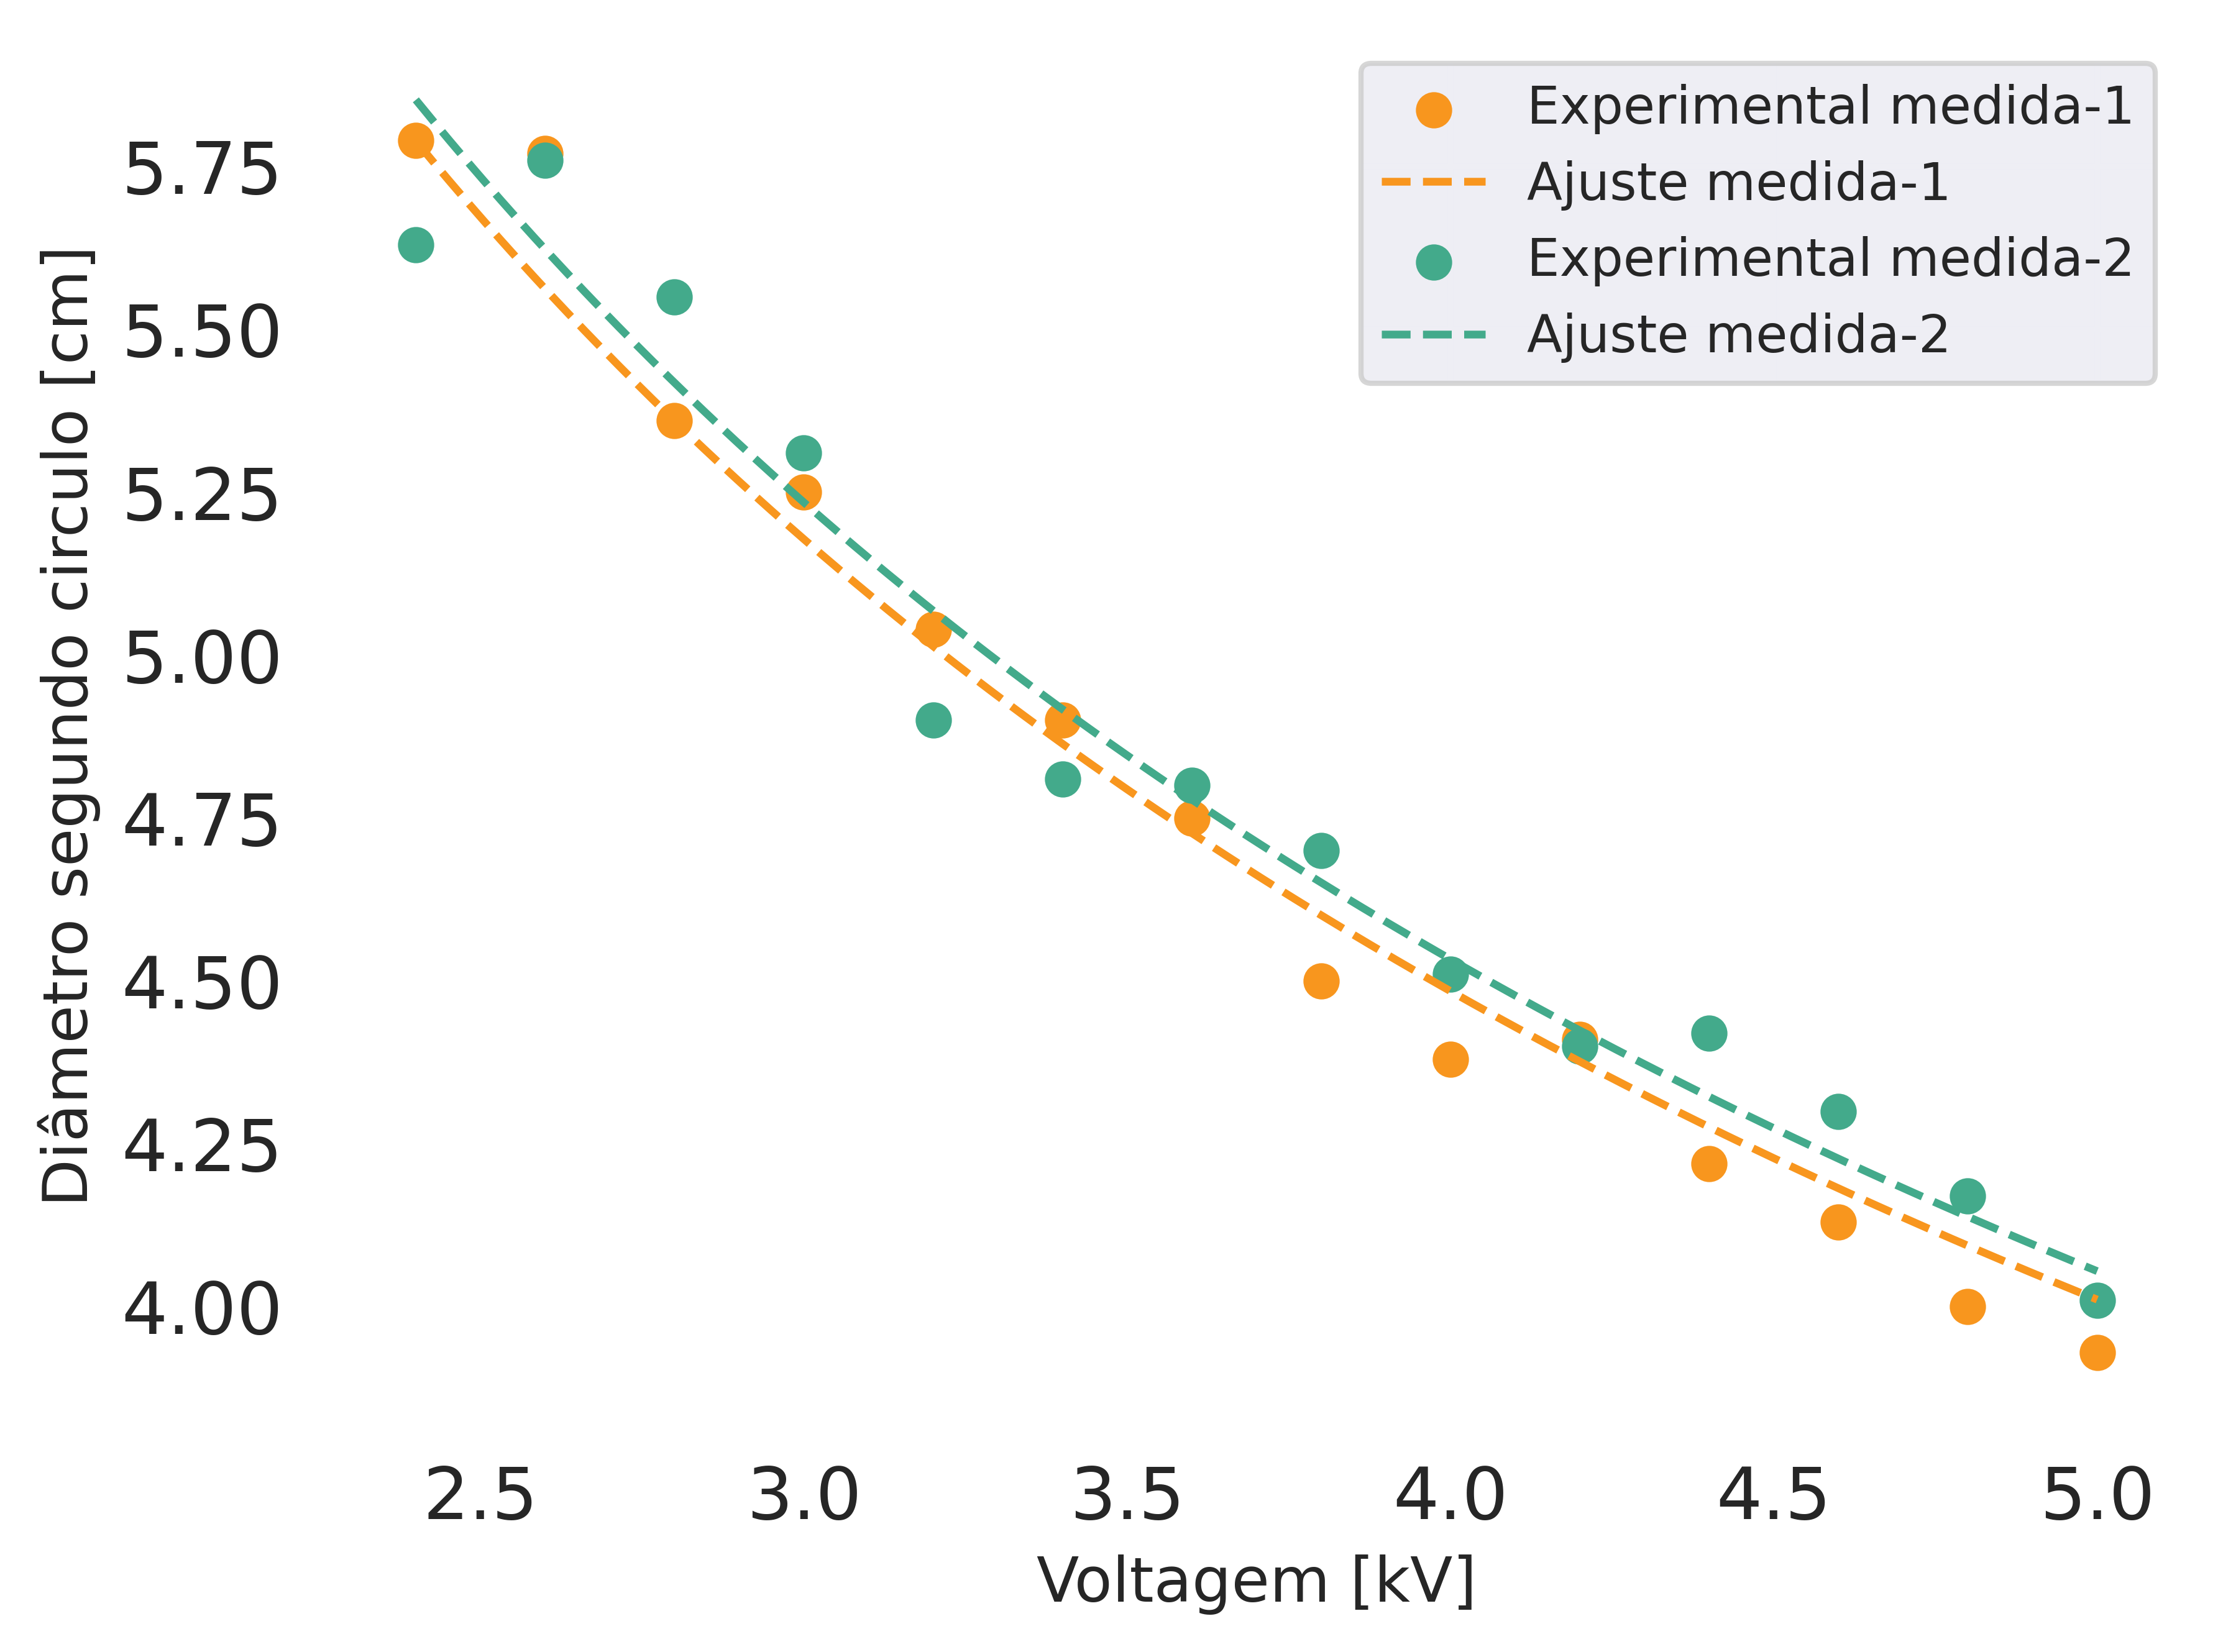
\includegraphics[width=0.75\textwidth,height=0.75\textheight,keepaspectratio]{figuras/fit2.png}\par
        % {\scriptsize Fonte: Elabora pelo autor.}
        \end{figure}
        \end{center}
    
\end{frame}

\begin{frame}{Equação utilizada no ajuste de curva}
    
    Equação utilizada no ajuste de curva para os dados experimentais obtidos, curva Diametros [cm] $\times$ $V$ (Tensão) em [Volts], do primeiro e segundo padrão de Difração
    \begin{equation}
    r = \frac{l}{2d} \frac{h}{\sqrt{2 m e V}}
    \end{equation}

    onde usamos, para realizar o ajuste númerico,
    \begin{equation}
    r = \alpha V^{-1/2}
    \end{equation}

\end{frame}

\begin{frame}{Funcionamento do código utilizado na analise dos dados}

\centering
\begin{tikzpicture}[node distance=1.5cm, auto, thick, scale=0.7, every node/.style={scale=0.7}]
\tikzstyle{block} = [rectangle, draw, rounded corners, text centered, minimum width=5cm, minimum height=1cm]

\node[block] (entrada) {Entrada: dados experimentais ($2\cdot r$) e parâmetros ($d$, $l$, $V$)};
\node[block, below of=entrada] (calc1) {Cálculo de $\lambda_{Bragg} = \tfrac{2\cdot r \cdot d}{l}$ para cada $d$};
\node[block, below of=calc1] (calc2) {Cálculo teórico de $\lambda_{Broglie} = \sqrt{\tfrac{150}{V}} \cdot 10^{-10}$};
\node[block, below of=calc2] (comp) {Comparação: encontra $\lambda_{Broglie}$ mais próximo de cada $\lambda_{Bragg}$};
\node[block, below of=comp] (saida) {Saída: melhor $d$, melhor $V$, diferença mínima};

\draw[->] (entrada) -- (calc1);
\draw[->] (calc1) -- (calc2);
\draw[->] (calc2) -- (comp);
\draw[->] (comp) -- (saida);

\end{tikzpicture}

\vspace{0.5cm}
\textbf{Resumo:} O código busca a correspondência entre teoria ($\lambda_{Broglie}$) e experimento ($\lambda_{Bragg}$), 
determinando a melhor voltagem e distância interplanar para cada medida.


\end{frame}

%------------------------------------------------


\begin{frame}{Resultados}

        \begin{center}
        \begin{figure}
        \caption{Comparação entre $\lambda_{Broglie}$ e $\lambda_{Bragg}$ (normalizados)}
        \vspace*{-0.25cm}
        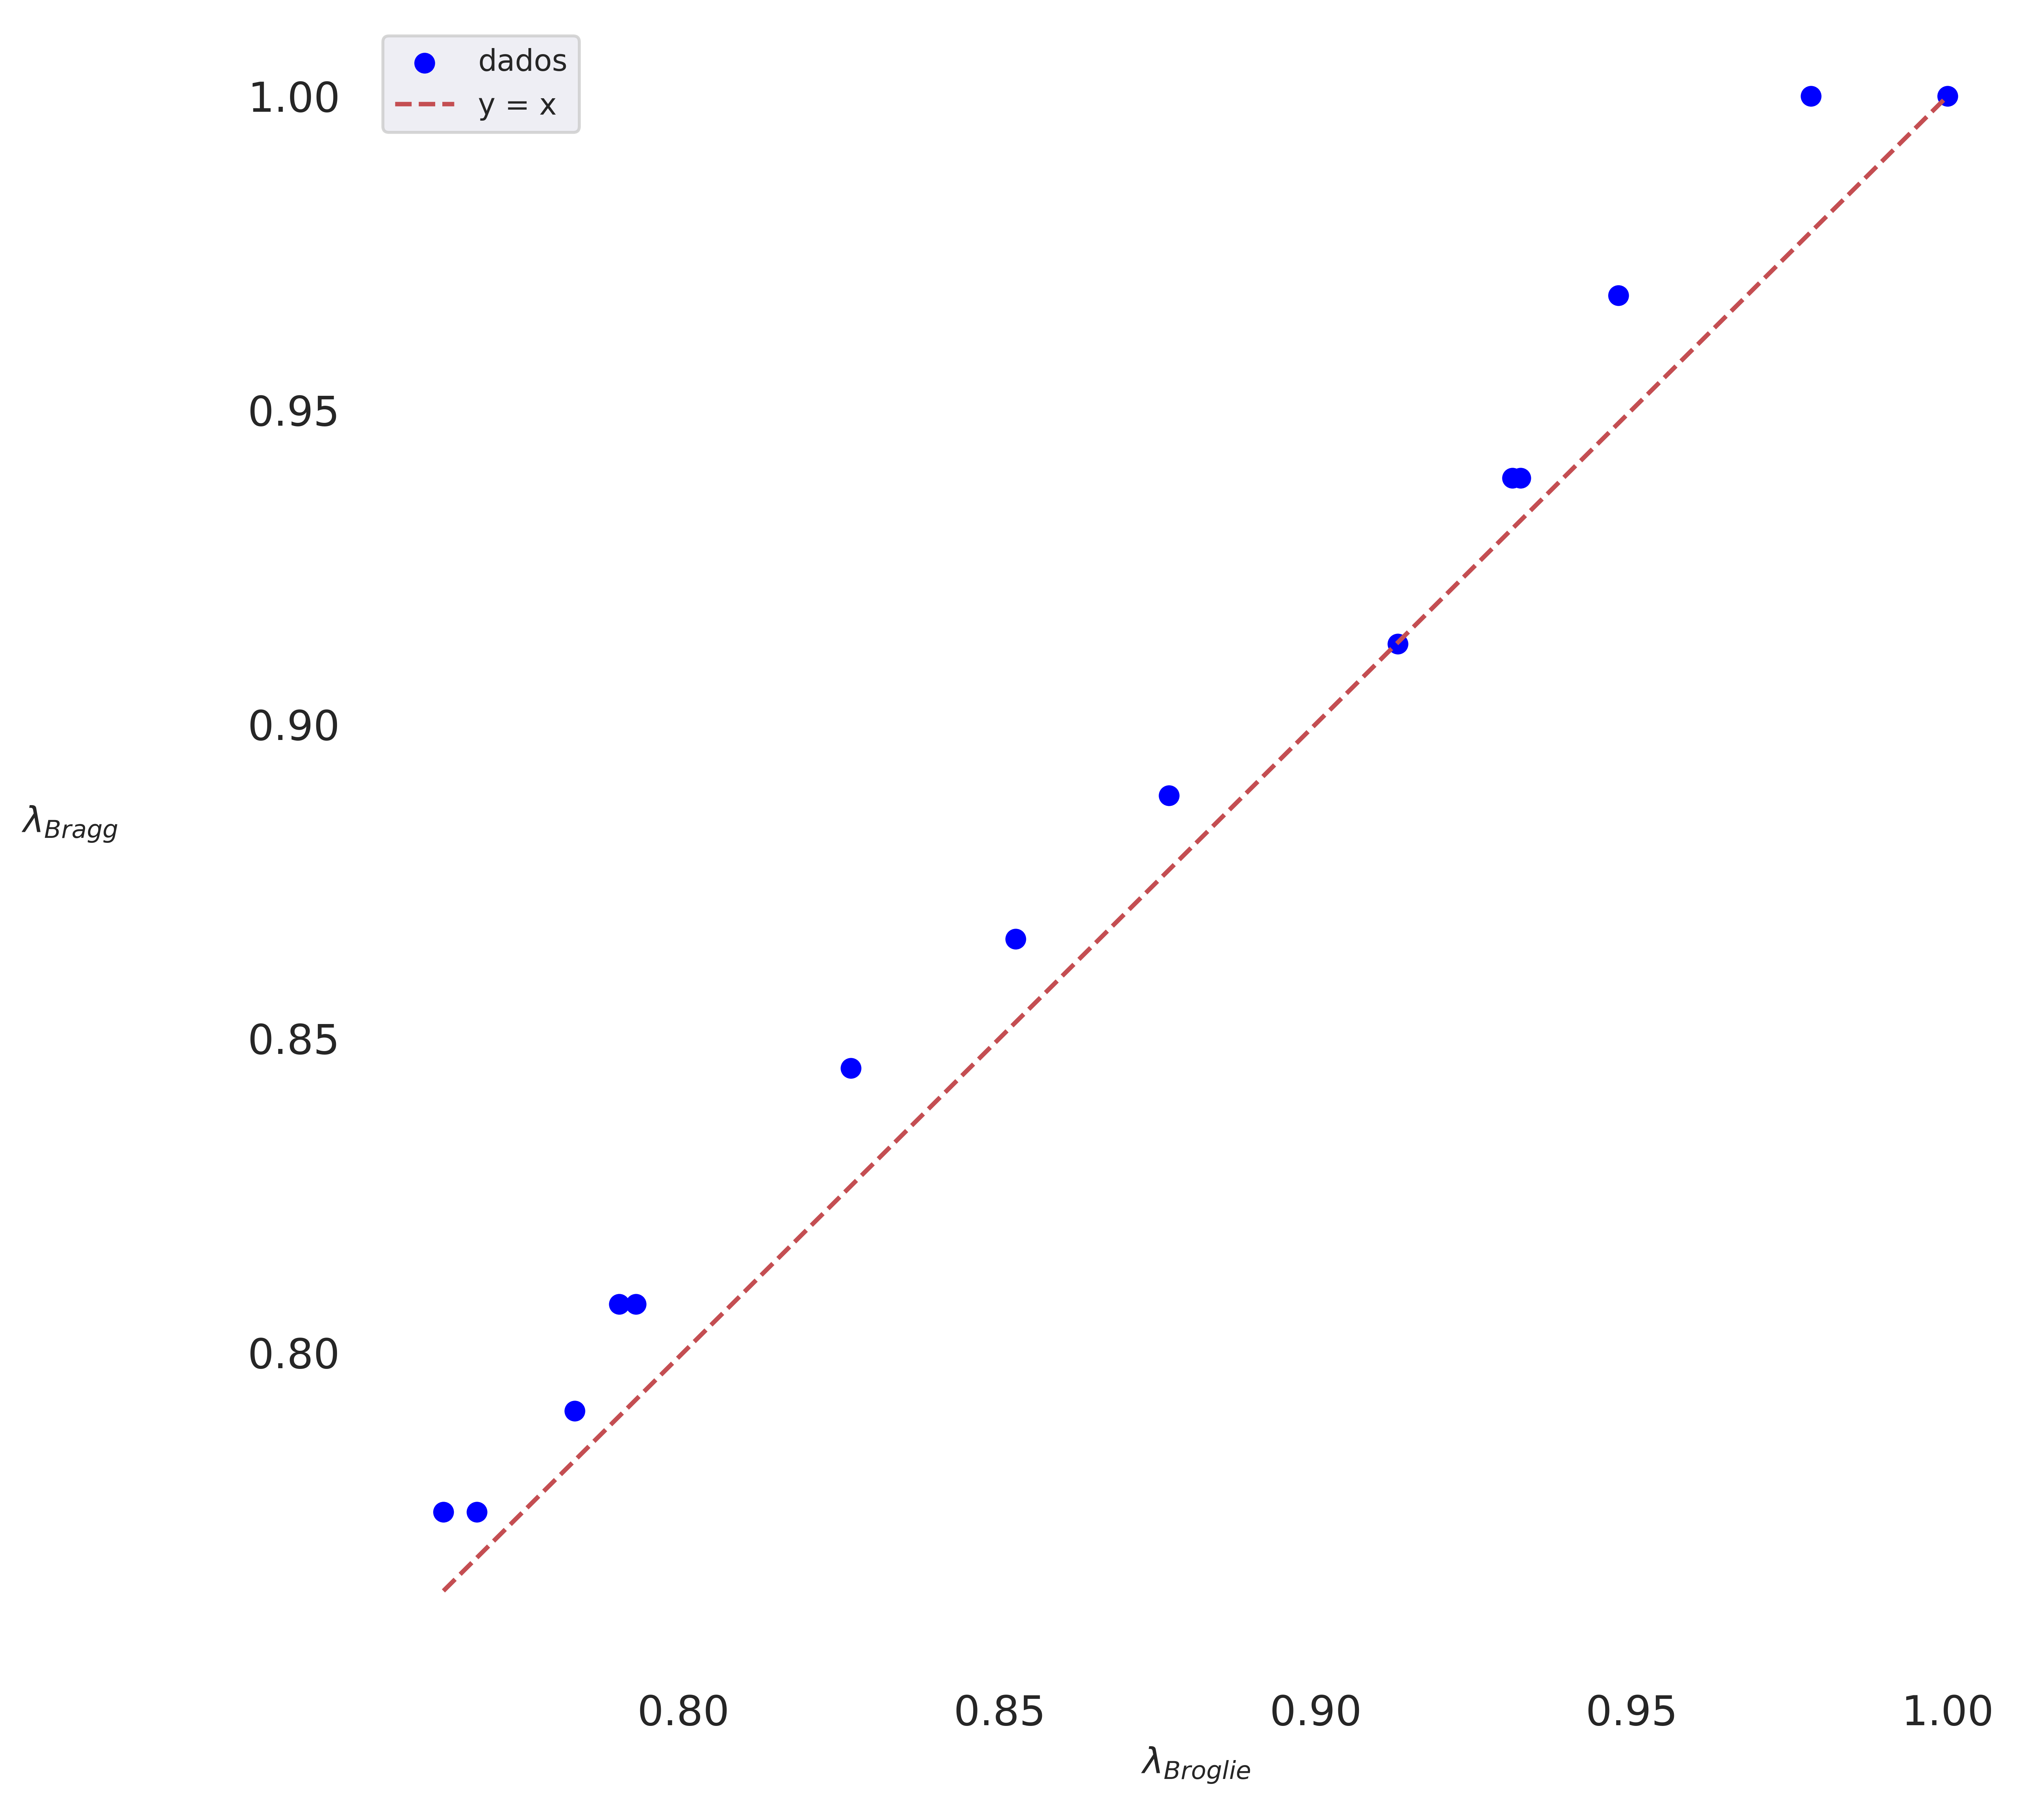
\includegraphics[width=0.75\textwidth,height=0.75\textheight,keepaspectratio]{figuras/plot1.png}\par
        % {\scriptsize Fonte: Elabora pelo autor.}
        \end{figure}
        \end{center}
    
\end{frame}

\begin{frame}{Resultados}

        \begin{center}
        \begin{figure}
        \caption{Diferença entre $\lambda_{Bragg}$ e $\lambda_{Broglie}$ (normalizados)}
        \vspace*{-0.25cm}
        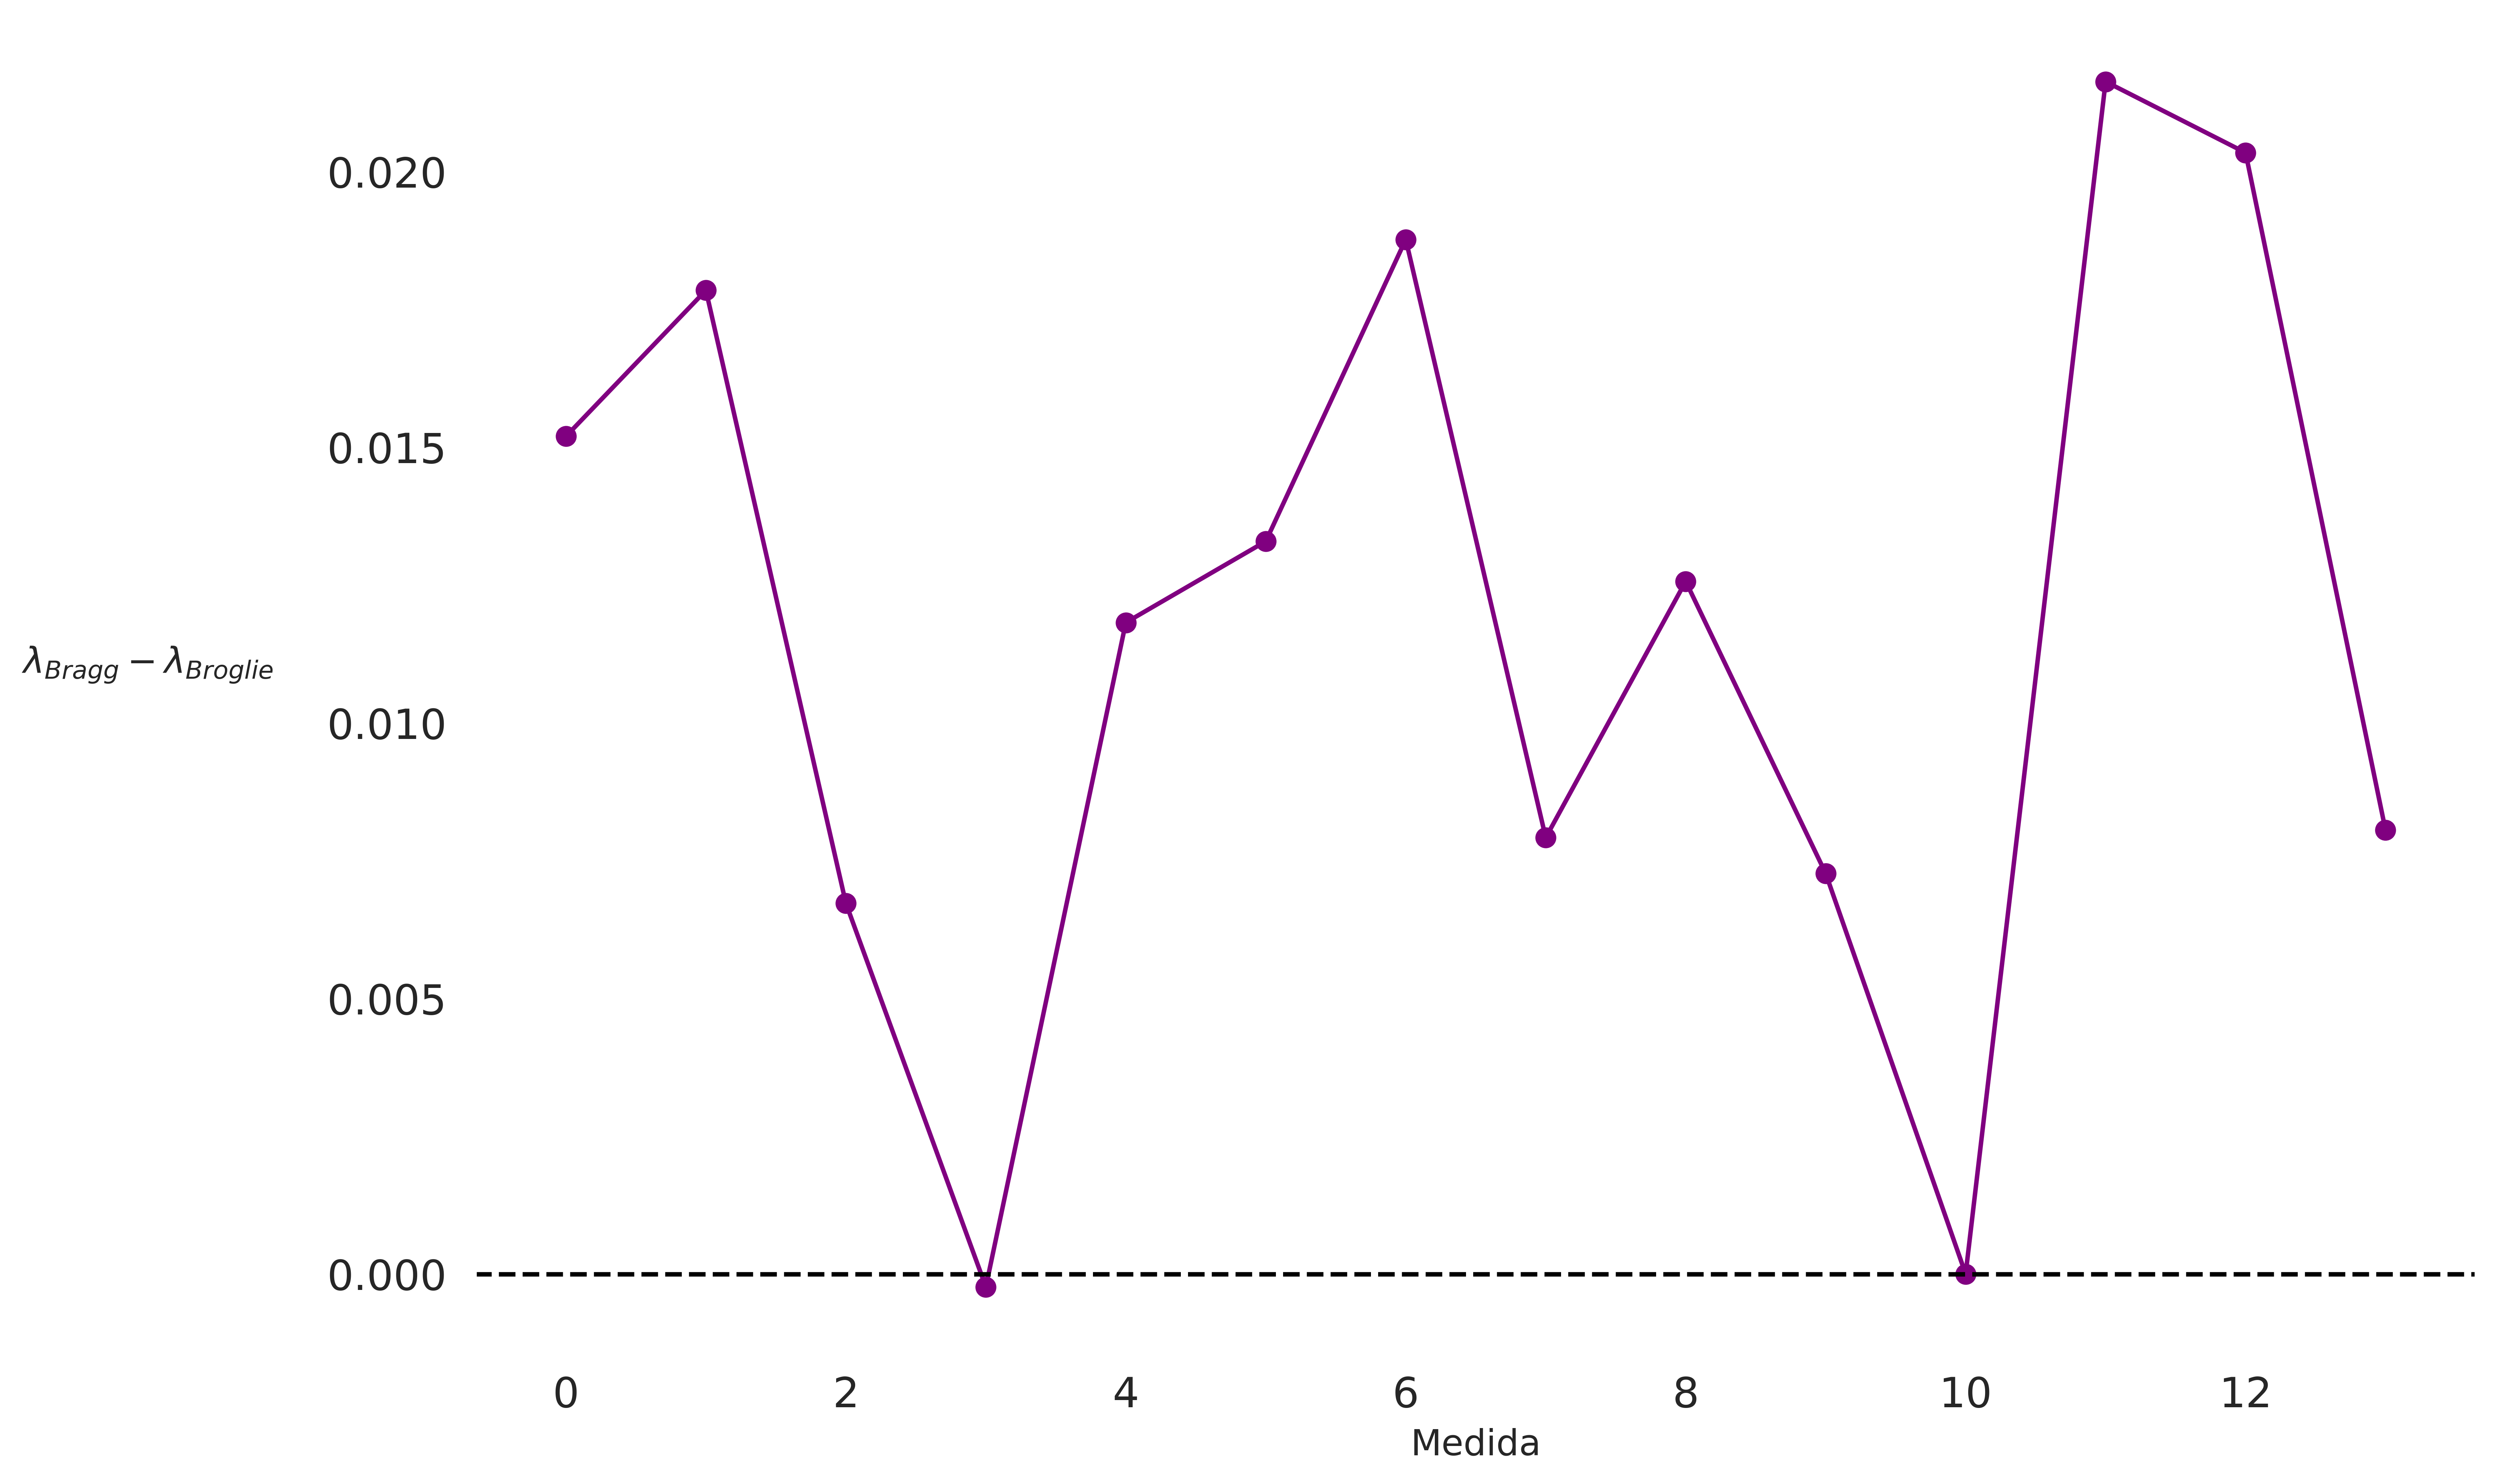
\includegraphics[width=0.75\textwidth,height=0.75\textheight,keepaspectratio]{figuras/plot3.png}\par
        % {\scriptsize Fonte: Elabora pelo autor.}
        \end{figure}
        \end{center}
    
\end{frame}

\begin{frame}{Distâncias
interplanares do policristal de grafite}

    \begin{table}[h!]
    \centering
    \scalebox{1.50}{
    \begin{tabular}{c c}
    \hline
    Índice & \(d \, (\text{\AA})\) \\
    \hline
    1 & 2.130 \\
    2 & 1.230 \\
    3 & 0.805 \\
    4 & 0.591 \\
    5 & 0.465 \\
    \hline
    \end{tabular}}
    \caption{Valores $d$ (distâncias
interplanares) em ångströms (\AA)}
    \end{table}
    


\end{frame}

\begin{frame}{Distâncias
interplanares associadas ao comprimento de onda de Bragg}

    \begin{table}[h!]
    \centering
    \scalebox{0.90}{
    \begin{tabular}{c c c}
    \hline
    Medida & $\lambda_{Bragg}$ (\AA) & $d$ (\AA) \\
    \hline
    0  & $0.1806$ & $0.4650$ \\
    1  & $0.1806$ & $0.4650$ \\
    2  & $0.2100$ & $0.5910$ \\
    3  & $0.2041$ & $0.5910$ \\
    4  & $0.1987$ & $0.5910$ \\
    5  & $0.1936$ & $0.5910$ \\
    6  & $0.1890$ & $0.5910$ \\
    7  & $0.1768$ & $0.5910$ \\
    8  & $0.1732$ & $0.5910$ \\
    9  & $0.1732$ & $0.5910$ \\
    10 & $0.2236$ & $0.8050$ \\
    11 & $0.2236$ & $0.8050$ \\
    12 & $0.2165$ & $0.8050$ \\
    13 & $0.2100$ & $0.8050$ \\
    \hline
    \end{tabular}}
    \caption{Valores de $\lambda_{Bragg}$ e $d$ (distâncias
interplanares), ambos em ångströms (\AA), para cada medida.}
    \end{table}
    

\end{frame}


\begin{frame}{Resultados}

        \begin{center}
        \begin{figure}
        \caption{Curva $\lambda_{Broglie}$ (valores melhor ajustados) $\times$ $\frac{1}{\sqrt{V}}$}
        \vspace*{-0.25cm}
        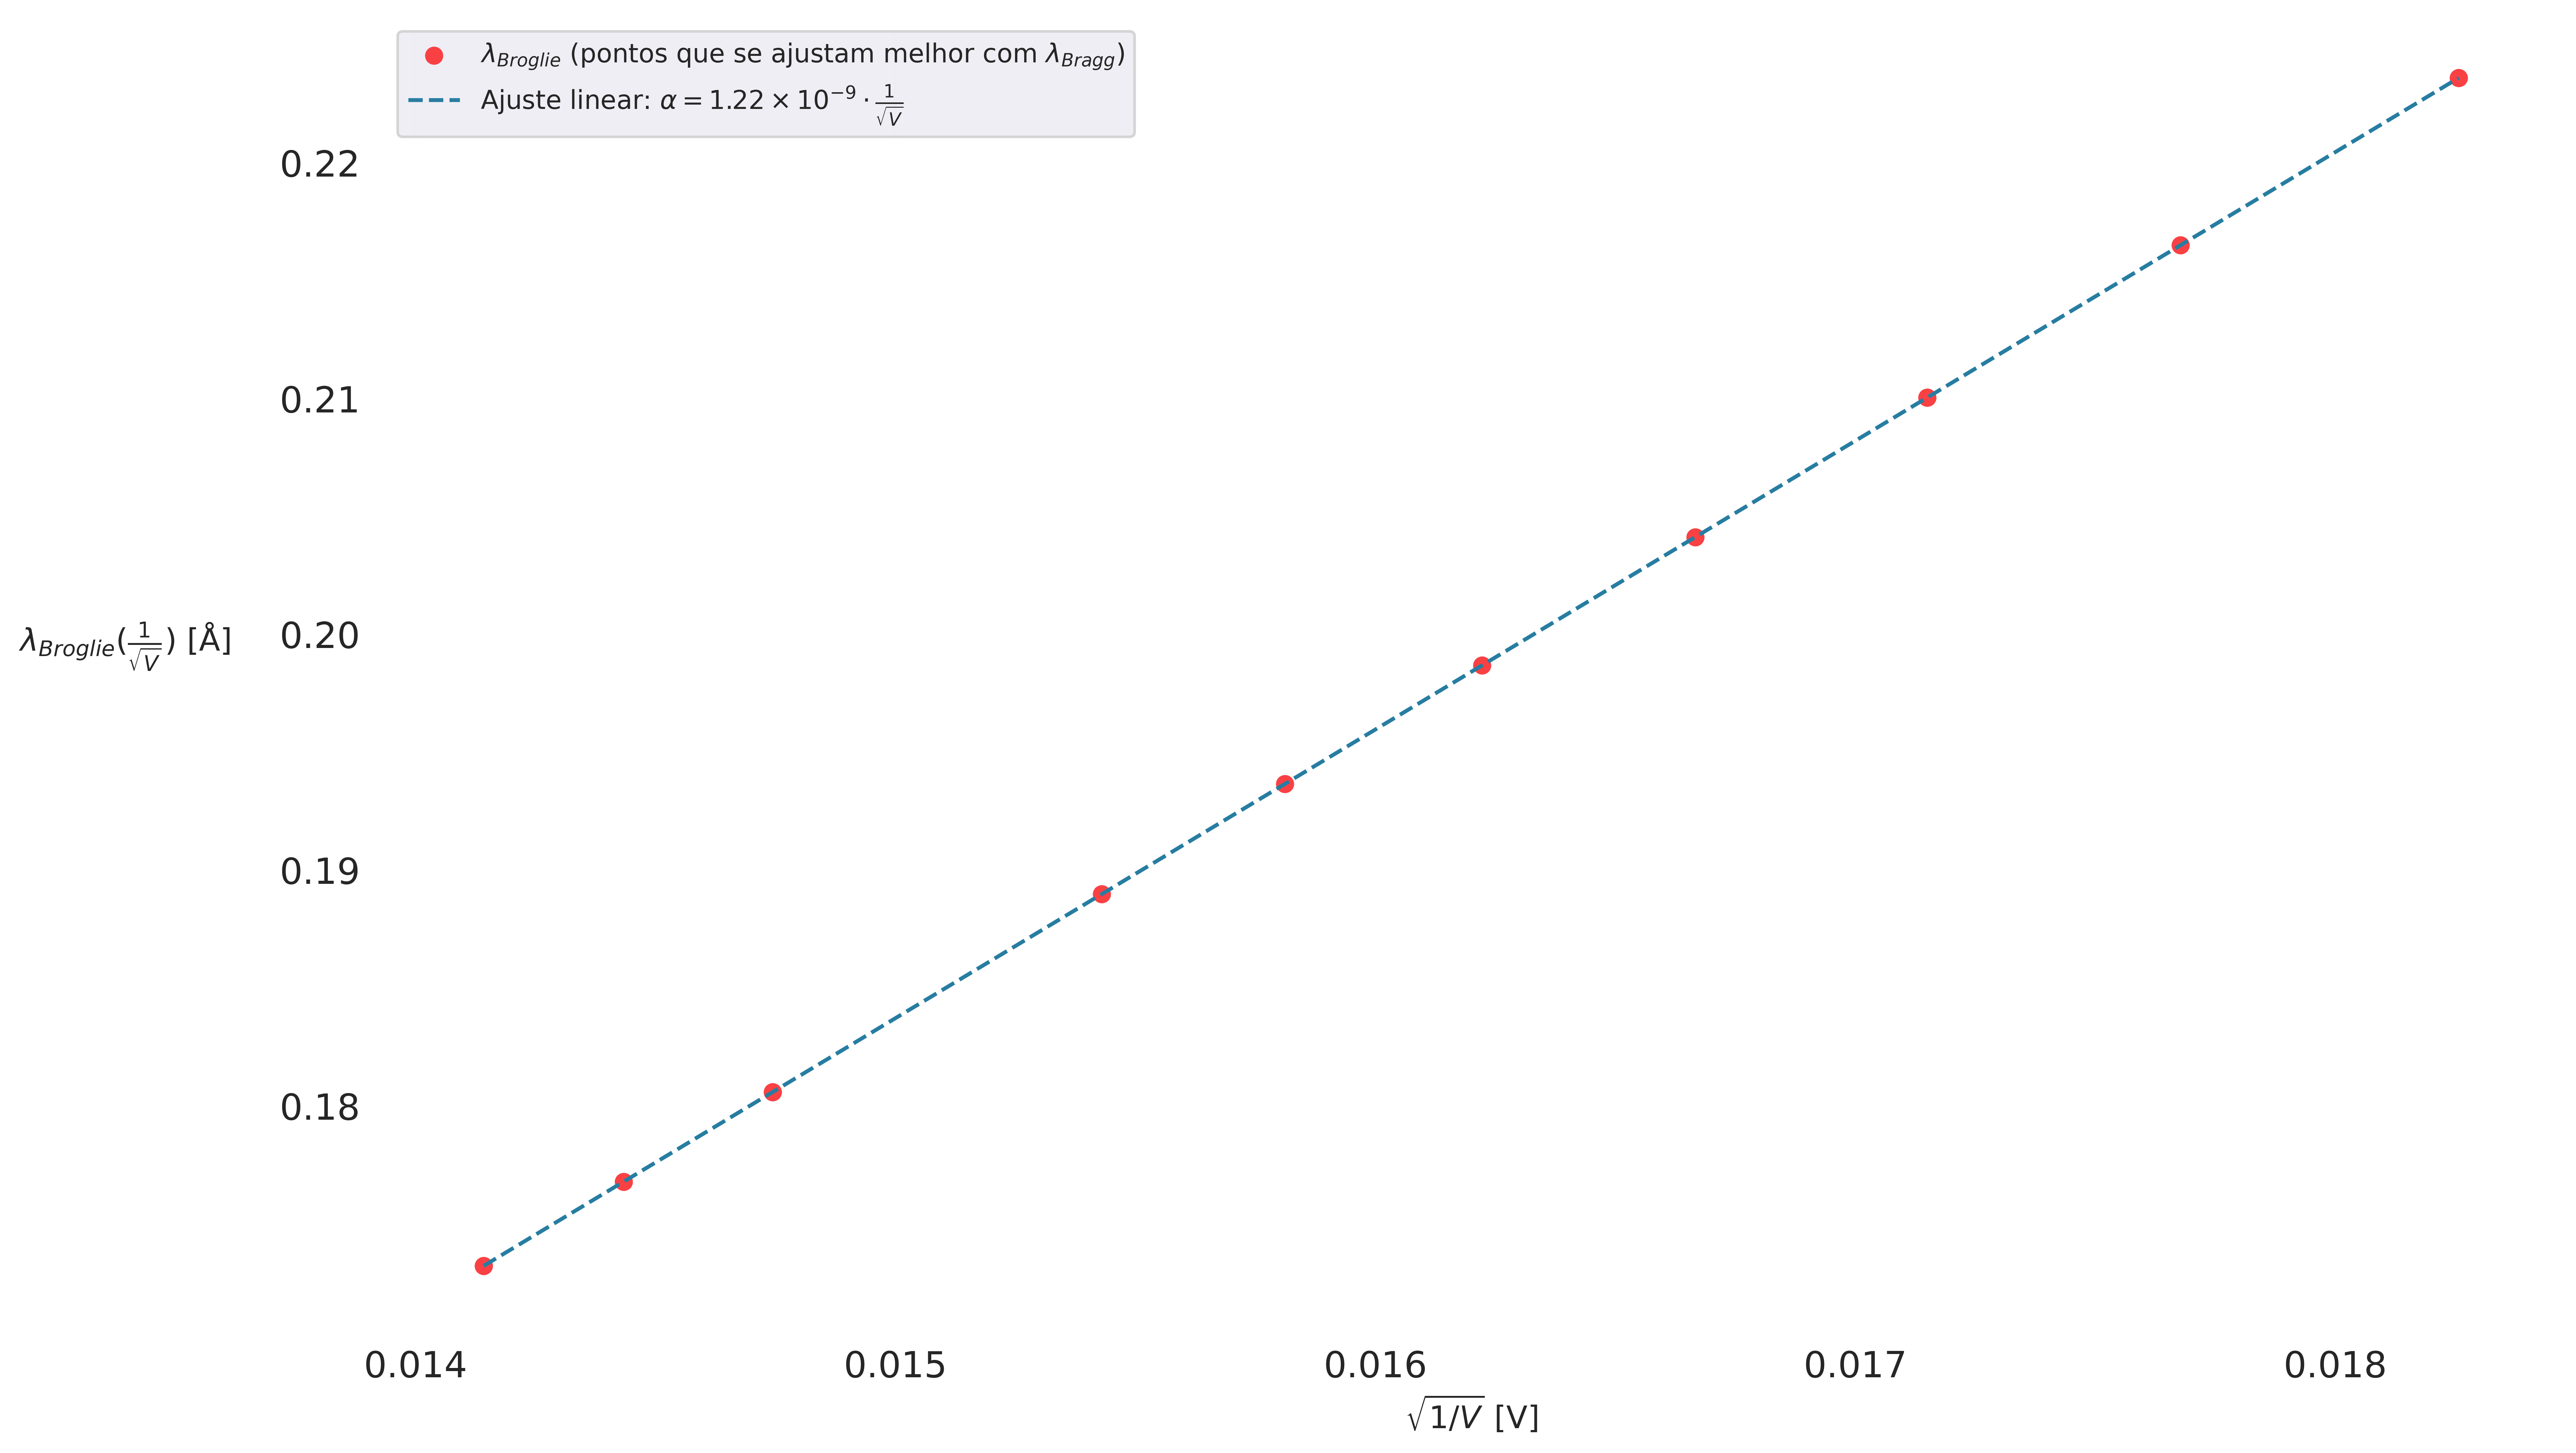
\includegraphics[width=0.75\textwidth,height=0.75\textheight,keepaspectratio]{figuras/fit3.png}\par
        % {\scriptsize Fonte: Elabora pelo autor.}
        \end{figure}
        \end{center}
    
\end{frame}

\begin{frame}{Econtrando o valor de $h$}

Encontraremos o valor de $h$ a partir do ajuste dos dados experimentais, temos:
\begin{equation}
\lambda_{Broglie} = \frac{h}{\sqrt{2 m e}} \, V^{-\tfrac{1}{2}} = \alpha \cdot V^{-\tfrac{1}{2}}
\end{equation}
\indent Isso posto,

\begin{equation}
\alpha := \frac{h}{\beta} \quad ; \quad \beta := \sqrt{2 m e}
\end{equation}
\indent Dessa forma, isolando $h$, temos:
\begin{equation}
h = \alpha \cdot \beta
\end{equation}
com os valores de $\alpha = 1.224744 \times 10^{-09}$ $\pm 5.1885 \times 10^{-25}
$ e $\beta = 5.402747 \times 10^{-25}$ conhecidos, podemos encontrar $h$.

\begin{equation}
        h =  6.616988 \times 10^{-34} \pm 5.1885 \times 10^{-25} \text{[J$\cdot$s]}
\end{equation}

\end{frame}

